\title{Changes on CRAN}
\subtitle{2022-01-01 to 2022-03-31}
\author{by Kurt Hornik, Uwe Ligges and Achim Zeileis}
\maketitle

\sloppy

\inputencoding{utf8}

In the past 3 months, 617 new packages were added to the CRAN package
repository.  86 packages were unarchived and 307 were archived.  The
following shows the growth of the number of active packages in the CRAN
package repository:

\begin{figure}[h]
  \centering
  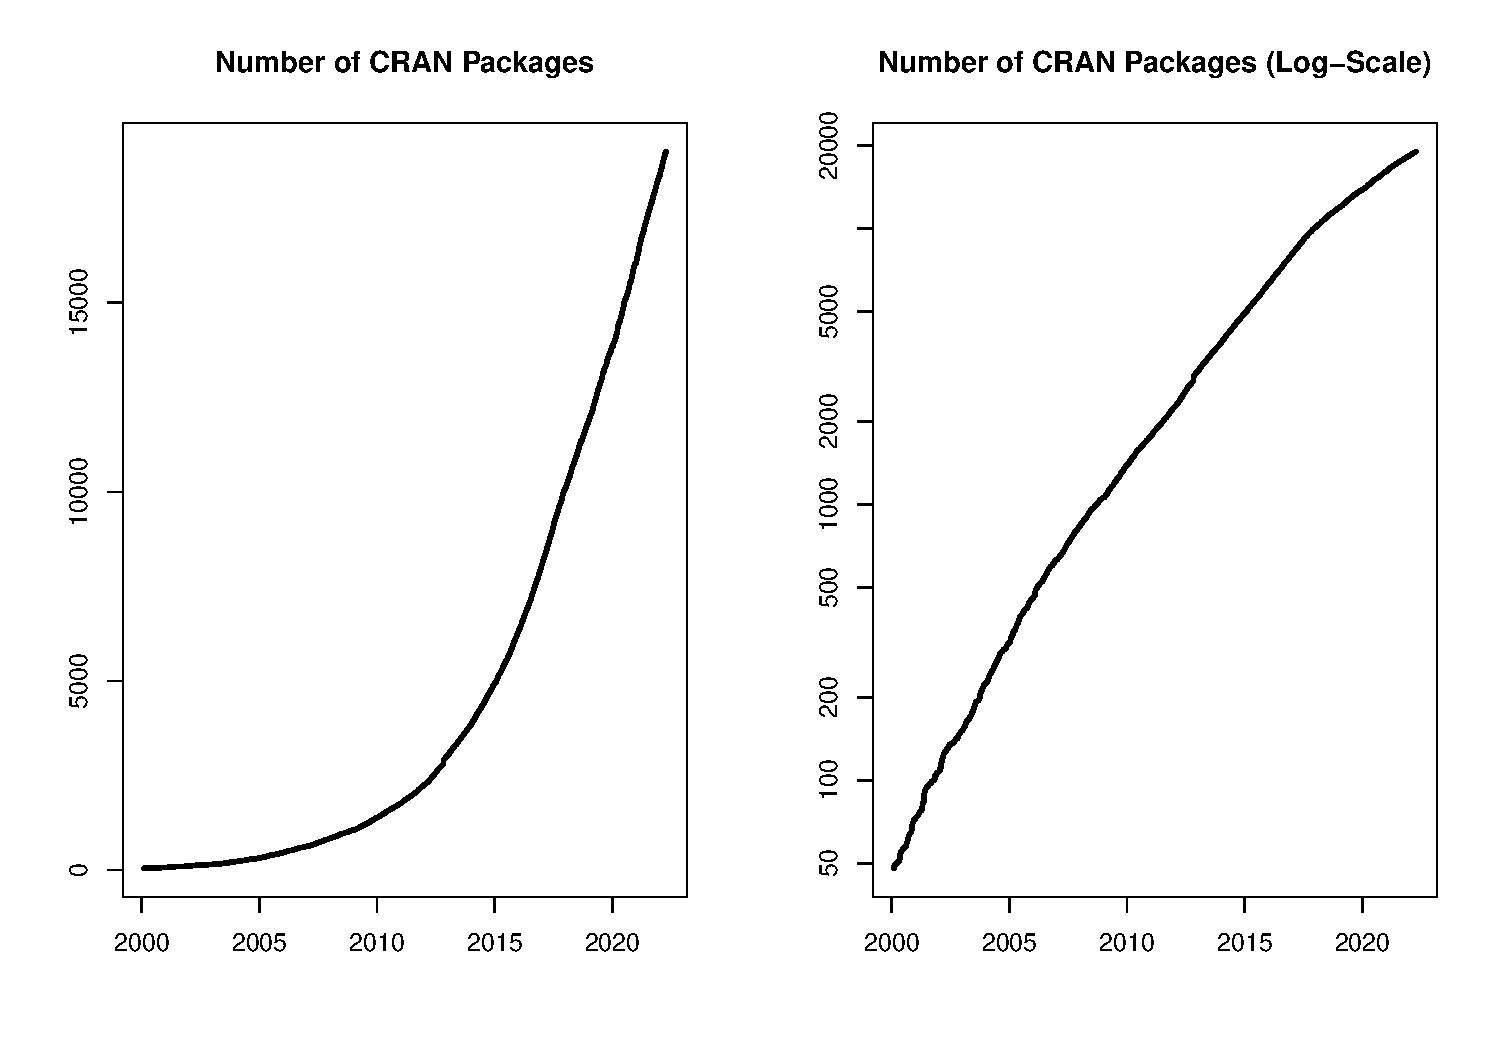
\includegraphics[width=5in]{cran_growth}
\end{figure}

\noindent
On 2022-03-31, the number of active packages was around 18924.

\subsection{Changes in the CRAN Repository Policy}

%% cd ~/src/org/R-project/R-dev-web/CRAN/Policy
%% svn diff -r{2022-01-01}:{2022-03-31}

The
\href{https://CRAN.R-project.org/web/packages/policies.html}{Policy}
now says the following:
\begin{itemize}
 \item (\strong{Using external C/C++/Fortran libraries.})
  Where a package
wishes to make use of a library not written solely for the package, the
package installation should first look to see if it is already installed
and if so is of a suitable version.  In case not, it is desirable to
include the library sources in the package and compile them as part of
package installation.  If the sources are too large, it is acceptable to
download them as part of installation, but do ensure that the download
is of a fixed version rather than the latest.  Only as a last resort
and with the agreement of the CRAN team should a package download
pre-compiled software.

On Windows and macOS static libraries must be used. A separate document,
\href{https://CRAN.R-project.org/web/packages/external_libs.html}{External
  Libraries for CRAN packages}, covers what external libraries are or
could be made available.
\end{itemize}

\subsection{CRAN package submissions}

During the first 4 months of 2022 (January 2022 to April 2022), CRAN 
received 9601 package submissions.
For these, 17170 actions took place of which 11232 (65\%) were auto
processed actions and 5938 (35\%) manual actions.

Minus some special cases, a summary of the auto-processed and manually
triggered actions follows:
\begin{center}
\begin{tabular}{l|rrrrrrrr}
           &archive& inspect& newbies& pending& pretest& publish& 
recheck& waiting\\ \hline
   auto    &  2391 &   2716 &   1392 &      0 &      0 &   3018 &   1017 
&    698\\
   manual  &  1893 &     93 &    487 &    323 &    106 &   2232 &    637 
&    167
\end{tabular}
\end{center}

These include the final decisions for the submissions which were
\begin{center}
\begin{tabular}{l|rr}
action & archive        & publish\\ \hline
auto   &   2232 (23.9\%)  & 2479 (26.5\%)\\
manual &   1870 (20.0\%)  & 2758 (29.5\%)
\end{tabular}
\end{center}
where we only count those as \emph{auto} processed whose publication or
rejection happened automatically in all steps.


A new team member, Viktoria Wimmer, joined the CRAN submission team. 
Welcome, Viktoria.
Unfortunately, Julia Haider left the CRAN submission team after 
processing 3517 incoming submissions. Thanks a lot!

\subsection{CRAN mirror security}

%% ~/Work/R/CRAN_Admin/cran_secure_http_and_rsync.R

Currently, there are 102 official CRAN mirrors, 81 of which provide both
secure downloads via \samp{https} \emph{and} use secure mirroring from
the CRAN master (via rsync through ssh tunnels).  Since the R 3.4.0
release, \code{chooseCRANmirror()} offers these mirrors in preference to
the others which are not fully secured (yet).

\subsection{CRAN Task View Initiative}

The transition of the established task views to the new workflow on
GitHub (\url{https://github.com/cran-task-views/ctv/}) that was
announced in the previous volume of the journal has been completed (see
also \url{https://twitter.com/AchimZeileis/status/1510945091980038145}).

Each task view now links to a GitHub repository where it is possible to
post issues and make pull requests for proposing improvements -- in
addition to sending e-mails to the maintainer address which is still
possible, of course.  Moreover, the task view web pages contain further
improvements like a citation, installation notes, and a streamlined
overview of core and regular (and currently archived) packages in the
task view.

Proposals of new task views are now also possible on GitHub. In fact, a 
few have already been made for the topics causal inference, genetics and 
genomics (as a follow-up to the orphaned and archived \emph{Genetics} and 
\emph{Phylogenetics} views), and sports analytics.

We look forward to further user contributions to the initiative!


\address{Kurt Hornik \\
  WU Wirtschaftsuniversit\"at Wien, Austria \\
  \email{Kurt.Hornik@R-project.org}}

\address{Uwe Ligges \\
  TU Dortmund, Germany \\
  \email{Uwe.Ligges@R-project.org}}

\address{Achim Zeileis \\
  Universit\"at Innsbruck, Austria \\
  \email{Achim.Zeileis@R-project.org}}

